\documentclass[tikz,border=9pt]{standalone}
\usepackage[T1]{fontenc}
\definecolor{espresso}{HTML}{98552C}
\definecolor{milk}{HTML}{476DB0}
\definecolor{cold}{HTML}{16877F}
\definecolor{sugar}{HTML}{AD4280}
\definecolor{decaf}{HTML}{7B7130}
\begin{document}
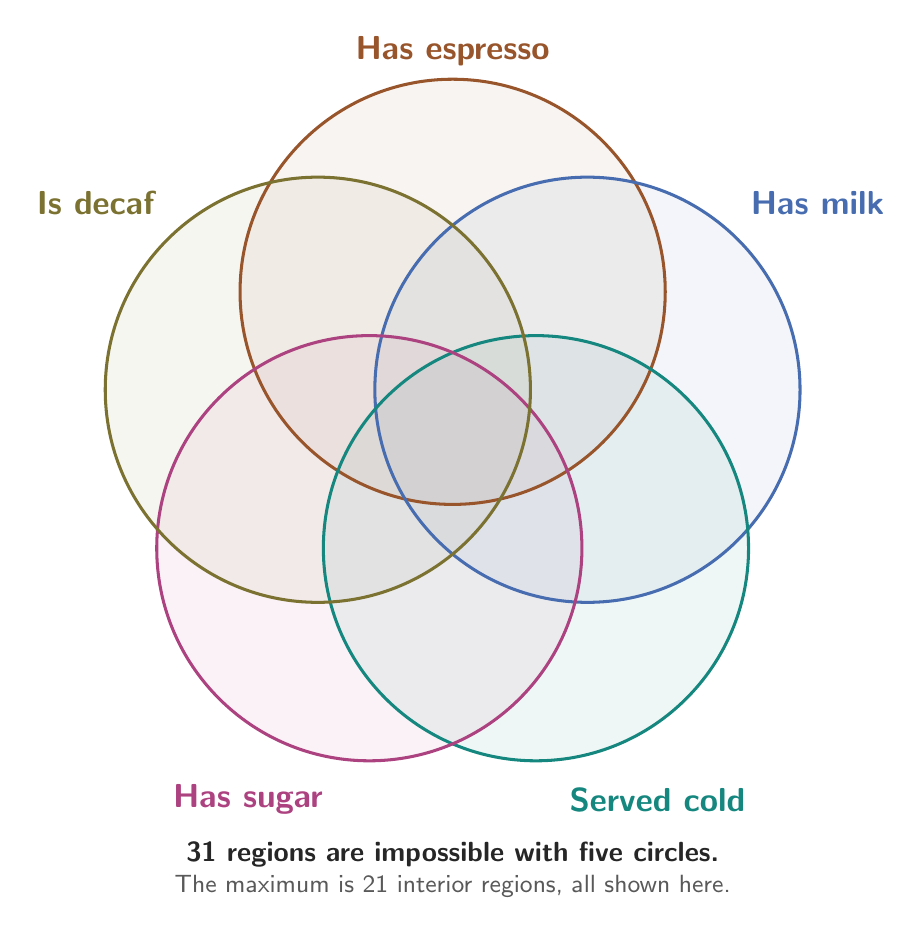
\begin{tikzpicture}[font=\sffamily, line width=1.1pt]
  % Five circles have at most n(n-1)+2 = 22 planar faces:
  % one exterior face and 21 interior faces. A 5-set Venn diagram
  % needs 31 interior faces, so the requested circle-only Venn is impossible.
  % Equal circles on a regular pentagon attain the 21-interior-face bound.
  \foreach \angle/\colour in {90/espresso,18/milk,-54/cold,-126/sugar,162/decaf}{
    \fill[\colour,fill opacity=.065] (\angle:1.8) circle[radius=2.7];
  }
  \foreach \angle/\colour in {90/espresso,18/milk,-54/cold,-126/sugar,162/decaf}{
    \draw[\colour] (\angle:1.8) circle[radius=2.7];
  }
  \node[text=espresso,font=\sffamily\bfseries\large] at (0,4.85) {Has espresso};
  \node[text=milk,font=\sffamily\bfseries\large,anchor=south west] at (3.65,2.65) {Has milk};
  \node[text=decaf,font=\sffamily\bfseries\large,anchor=south east] at (-3.65,2.65) {Is decaf};
  \node[text=cold,font=\sffamily\bfseries\large] at (2.6,-4.65) {Served cold};
  \node[text=sugar,font=\sffamily\bfseries\large] at (-2.6,-4.65) {Has sugar};
  \node[font=\sffamily\bfseries, text=black!85] at (0,-5.35)
    {31 regions are impossible with five circles.};
  \node[font=\sffamily\small, text=black!65] at (0,-5.75)
    {The maximum is 21 interior regions, all shown here.};
\end{tikzpicture}
\end{document}
